% !TEX root = 99_main.tex

Buildings are at the heart of society and currently account for 32\% of global final energy consumption and 19\% of energy related greenhouse gas emissions \cite{IPCC}. Nevertheless, the building sector has a 50-90\% emission reduction potential using existing technologies \cite{IPCC}. Within this strategy, building integrated photovoltaics (BIPV) have the potential of providing a substantial segment of a building's energy needs \cite{defaix2012technical}. Even the photovoltaic (PV) industry has identified BIPV as one of the four key factors for the future success of PV \cite{raugei2009life}. 

%Recent developments regarding efficiency and costs of thin film BIPV technologies, in particular, CIGS, have brought new design possibilities \cite{NREL} \cite{kushiya2014cis} \cite{kaelin2004low} \cite{jelle2012building}. Their lightweight nature and customisable shapes allow for easier and more aesthetically pleasing integration into the building envelope. In addition, less power is required to actuate them, thus facilitating the development of dynamic envelope elements \cite{rossi2012adaptive}. \\


Dynamic building envelopes have gained interest in recent years because they can save energy by controlling direct and indirect radiation into the building, while still responding to the desires of the user \cite{loonen2013climate}. This mediation of solar insolation offers a reduction in heating / cooling loads and an improvement of daylight distribution \cite{rossi2012adaptive}. Interestingly, the mechanics that actuate dynamic envelopes couples seamlessly with the mechanics required for facade integrated PV solar tracking. 

Previous BIPV research analyses electricity production and building energy demand for static BIPV shading systems \cite{mandalaki2012assessment} \cite{yoo2011available} \cite{freitas2015maximizing} \cite{jayathissa2015abs}. This paper expands on this work by analysing dynamic PV shading systems, while also taking into account mutual shading amongst modules and its effect on PV electricity generation. The approach allows us to reduce efficiency degradation due to partial shading of PV modules \cite{hofer2015PVSEC}.%This paper expands on this work by analysing dynamic PV shading systems, while also taking into account mutual shading amongst modules. This is particularly important for BIPV systems \cite{hofer2015PVSEC}. 

The work presented in this paper is applied in the context of the Adaptive Solar Facade (ASF) project \cite{nagy2015frontiers}. The ASF is a lightweight PV shading system composed of CIGS panels, that can be easily installed on any surface of new or existing buildings. This paper will present a methodology of simulating an ASF while simultaneously calculating the energy demand of the office space behind the facade.



% Within this study we analyse the trade-off in winter between PV generation and heating the room through solar insolation. Likewise in summer we discuss the trade-off between cooling and natural lighting. 

% The state of the art in this field is restricted to static shading devices \cite{yoo2011available} \cite{mandalaki2012assessment}. This paper presents a methodology to simulate a dynamic solar facade and calculate the electricity production in combination with the energy consumption of the building. 


% \begin{figure}
% \begin{center}
% 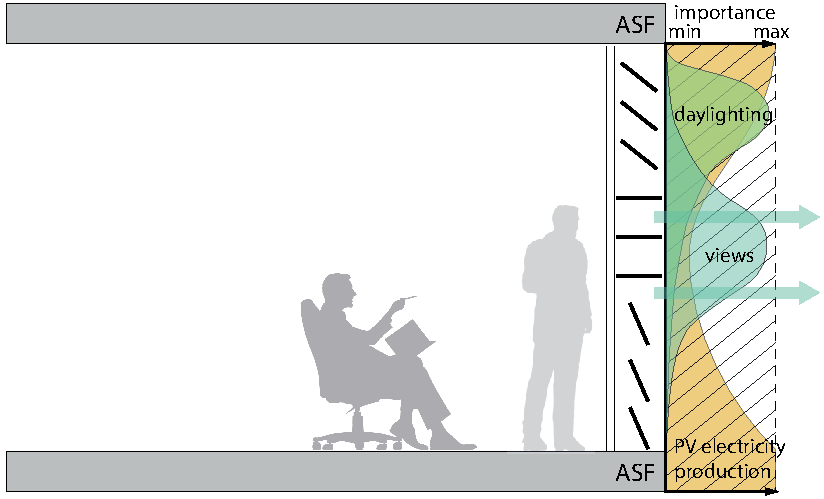
\includegraphics[width=8cm, trim= 0cm 0cm 0cm 0cm,clip]{facadeFunctions.pdf}
% \caption{The facade acting as a mediator between the interior and exterior environment, while fullfilling various functions \cite{nagy2015frontiers}}
% \label{fig:ASFschematic}
% \end{center}
% \end{figure}

% \begin{figure}
% \begin{center}
% \includegraphics[width=8cm, trim= 0cm 0cm 0cm 0cm,clip]{honr.jpg}
% \caption{An example of an ASF constructed at the House of Natural Resources \cite{nagy2015frontiers}}
% \label{fig:HoNR}
% \end{center}
% \end{figure}




